\graphicspath{{C:/Users/Kanis/FMF/RP/racunalniski-praktikum/08-prosojnice/slike/}} %namesto tega bi lahko v 17 napisal {slike/fig...}
\begin{frame}{Konstrukcija pravokotnice na premico $p$ skozi točko $T$}
	\begin{columns}
		\begin{column}{0.55\textwidth}
			\begin{itemize}[<+->]
				\item Dani sta premica $p$ in točka $T$.
				\item Nariši lok $k$ s središčem v $T$.
				\item Premico $p$ seče v točkah $A$ in $B$.
				\item Nariši lok $m$ s središčem v $A$.
				\item Nariši lok $n$ s središčem v $B$ in z enakim polmerom.
				\item Loka se sečeta v točki $C$.
				\item Premica skozi točki $T$ in $C$ je pravokotna na $p$.
			\end{itemize}
		\end{column}
		\begin{column}{0.45\textwidth}
			\centering
			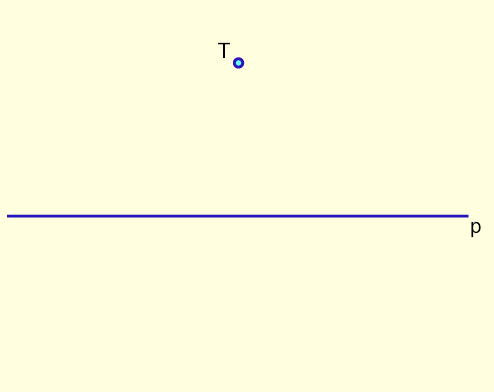
\includegraphics[width=50mm]{fig-1.png}<1>
	        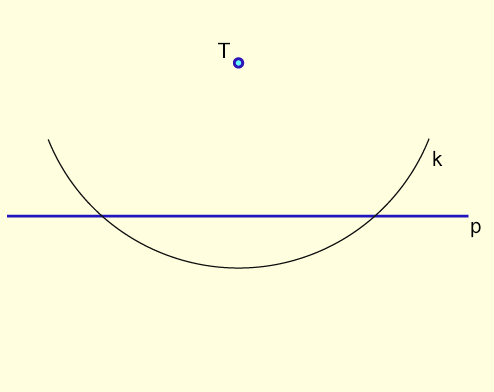
\includegraphics[width=50mm]{fig-2.png}<2>
	        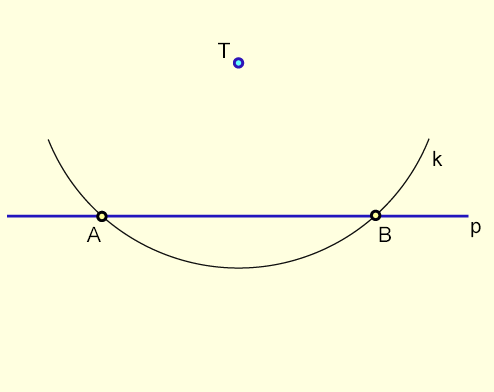
\includegraphics[width=50mm]{fig-3.png}<3>
	        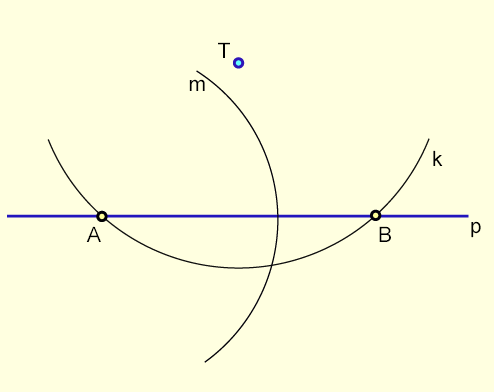
\includegraphics[width=50mm]{fig-4.png}<4>
	        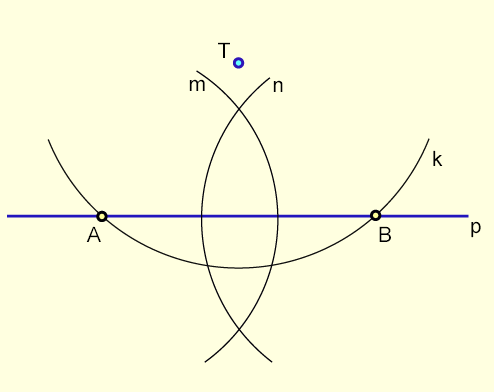
\includegraphics[width=50mm]{fig-5.png}<5>
	        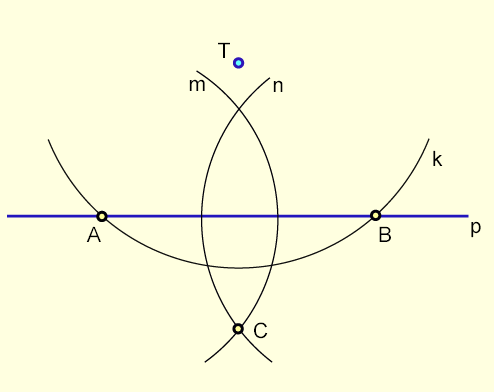
\includegraphics[width=50mm]{fig-6.png}<6>
	        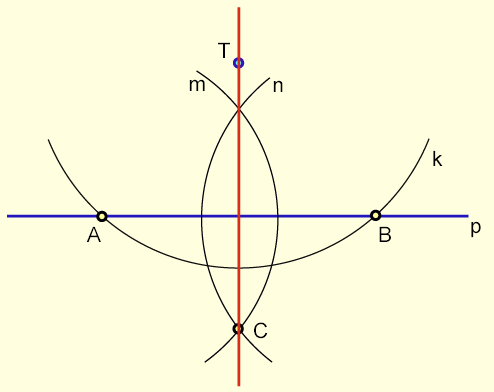
\includegraphics[width=50mm]{fig-7.png}<7>
		\end{column}
	\end{columns}
\end{frame}

\begin{frame}{Konstrukcija pravokotnice na premico $p$ skozi točko $T$}
	\begin{columns}
		\begin{column}{0.55\textwidth}
			\begin{itemize}
				\item<1-> Dani sta premica $p$ in točka $T$.
				\item<2-> Nariši lok $k$ s središčem v $T$.
				\item<3-> Premico $p$ seče v točkah $A$ in $B$.
				\item<4-> Nariši lok $m$ s središčem v $A$.
				\item<5-> Nariši lok $n$ s središčem v $B$ in z enakim polmerom.
				\item<6-> Loka se sečeta v točki $C$.
				\item<7-> Premica skozi točki $T$ in $C$ je pravokotna na $p$.
			\end{itemize}
		\end{column}
		\begin{column}{0.45\textwidth}
			\centering
			\begin{tikzpicture}
				\tikzmath{
					% Sliko smo naredili tako, da so točke A, B, T in C vse enako oddaljene
					% od presečišča premic; kot ATC je 45°.
					% Vsi krožni loki imajo radij 2.
					% Razdalja od točke T do premice p je tako 2*sin(45°).
					\t = 2*sin(45);
					% Razdalja začetka loka m do premice p
					% oz. razdalja točke T' levo in zgoraj od točke T do premice
					\tt = 2*sin(60);
					% Razdalja točke T' od navpične premice skozi T
					\td = \t-2*cos(60);
				}
				\only<7>\draw[red, very thick] (0,2) -- (0,-2);
				% Definicija točke T
				\coordinate [label={[blue, above]:$T$}] (T) at (0,{\t});
				% Risanje točke T
				\fill[blue] (T) circle (2pt);
				% Premica p
				\draw[blue, very thick] (-2,0) -- (2,0) node[right] {$p$};
				\pause
				% Definicija pomožne točke A' in risanje krožnega loka k, ki se začne v A'
				\coordinate (A') at ({-\tt},{\td});
				\draw[gray, thin] (A') arc[start angle=210, end angle=330, radius=2] node[right] {\scriptsize $k$};
				\pause
				% Točka A
				\coordinate [label=below left:{\scriptsize $A$}] (A) at ({-\t},0);
				\draw (A) circle (1.5pt);
				% Točka B
				\coordinate [label=below right:{\scriptsize $B$}] (B) at ({\t},0);
				\draw (B) circle (1.5pt);
				\pause
				\coordinate (T') at ({-\td},{-\tt});
				\draw[gray, thin] (T') arc[start angle=-60, end angle=60, radius=2] node[below left] {\scriptsize $m$};
				\pause
				\coordinate (T') at ({\td},{-\tt});
				\draw[gray, thin] (T') arc[start angle=240, end angle=120, radius=2] node[below right] {\scriptsize $n$};
				\pause
				\coordinate [label={[blue, below]:$C$}] (C) at (0,{-\t});
				\fill[blue] (C) circle (2pt);
				
			\end{tikzpicture}
		\end{column}
	\end{columns}
\end{frame}
%pause ne dela kot v rešitvah


% Spodnje je za nalogo 3.4.

% Naloga 3.4.1.: Narišite še točko B (skupaj z oznako)

% Naloga 3.4.2.: Definirajte točko T', v kateri se začne lok m in narišite lok m z oznako.
% Lok je definiran s točko, v kateri se lok začne (ne središče!), z začetnim in končnim kotom ter radijem.
% Koti so vedno podani enako: kot 0 je v smeri x osi in se veča v nasprotni smeri urinega kazalca.

% Naloga 3.4.3.: Definirajte točko T'' in narišite lok n z oznako.

% Naloga 3.4.4.: Definirajte in narišite točko C.

% Naloga 3.4.5.: Narišite premico skozi točki T in C.

% Konec vsebine za nalogo 3.4.


% Naloga 4
\begin{frame}{Graf funkcije s TikZ}
	\centering
	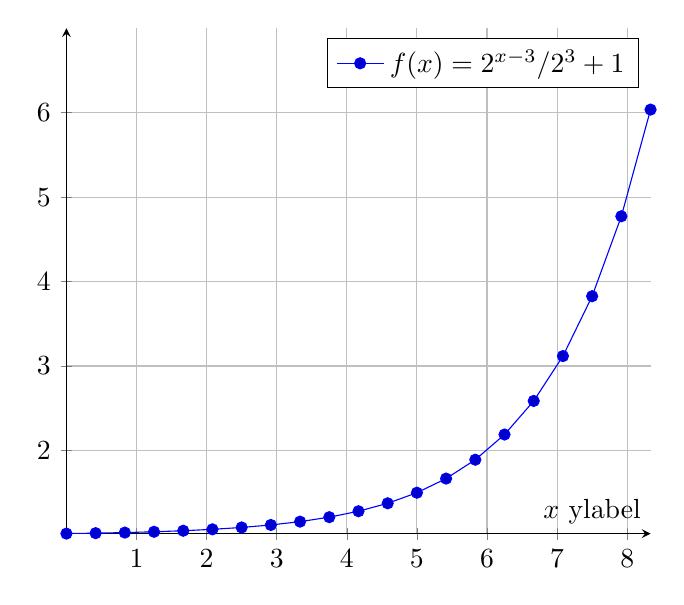
\begin{tikzpicture}
		\begin{axis}[
			axis lines = middle,
			domain = 0:10,
			width = 9cm,
			height = 8cm,
			xtick = {0, 1, 2, 3, 4, 5, 6, 7, 8},
			ytick = {0, 1, 2, 3, 4, 5, 6},
			xlabel=$x$
			ylabel=$y$
			ymin = -1,
			ymax = 7,
			grid = both
		]
			\addplot{2^(x - 3)/2^3 + 1};
			\addlegendentry{$f(x)=2^{x - 3}/2^3 + 1$}
		\end{axis}
	\end{tikzpicture}
\end{frame}